\documentclass[twoside]{article}


% ------
% Fonts and typesetting settings
\usepackage[sc]{mathpazo}
\usepackage[T1]{fontenc}
\linespread{1.05} % Palatino needs more space between lines
\usepackage{microtype}


% ------
% Page layout
\usepackage[hmarginratio=1:1,top=32mm,columnsep=20pt]{geometry}
\usepackage[font=it]{caption}
\usepackage{paralist}
\usepackage{multicol}

% ------
% Lettrines
\usepackage{lettrine}


% ------
% Abstract
\usepackage{abstract}
	\renewcommand{\abstractnamefont}{\normalfont\bfseries}
	\renewcommand{\abstracttextfont}{\normalfont\small\itshape}


% ------
% Titling (section/subsection)
\usepackage{titlesec}
\renewcommand\thesection{\Roman{section}}
\titleformat{\section}[block]{\large\scshape\centering}{\thesection.}{1em}{}


% ------
% Header/footer
\usepackage{fancyhdr}
	\pagestyle{fancy}
	\fancyhead{}
	\fancyfoot{}
	\fancyhead[C]{gUSE for cloud $\bullet$ March 2014 $\bullet$ SOMNO.Netz/ER-flow collaboration}
	\fancyfoot[RO,LE]{\thepage}


% ------
% Clickable URLs (optional)
\usepackage{hyperref}

% ------
% Maketitle metadata
\title{\vspace{-15mm}%
	\fontsize{24pt}{10pt}\selectfont
	\textbf{Evaluation of gUSE as workflow management system for a cloud-based sleep research platform}
	}	
\author{%
	\large
	\textsc{Christoph Jansen} \\[2mm]
	\normalsize	HTW Berlin \\
	\normalsize	\href{mailto:c.jansen@student.htw-berlin.de}{c.jansen@student.htw-berlin.de}
	\vspace{-5mm}
	}
\date{}



%%%%%%%%%%%%%%%%%%%%%%%%
\begin{document}

\maketitle
\thispagestyle{fancy}

\begin{abstract}
In sleep research multicentric studies produce a large amount of data like electrocardiography scans.
Various processing algorithms can be applied to these scans.

The QMROCT project introduced a cloud based data processing infrastructure with XNAT as data archive.
For the SOMNO.Netz sleep research project the workflow management system WS-PGRADE/gUSE is introduced to the architecture.
It supports more complex algorithms with multiple dependent jobs and is able to control resources of the OpenStack cloud.
Since WS-PGRADE/gUSE was originally developed for grid infrastructures, this paper describes how to set it up in a cloud based system and evaluates the productive usage in several aspects.

The paper concludes that WS-PGRADE/gUSE is generally working in cloud system, but is not able to handle errors produced by the cloud which results in instabilities and lacks of cloud specific features.
\end{abstract}

	

\begin{multicols}{2}


\section{Introduction}\label{introduction}

In sleep research large amounts of patient data are collected during sleep studies, also called polysomnographies.
In the course of the SOMNO.Netz project~\cite{krefting13} a data archiving and processing infrastructure is provided, to manage the data of 300 sleep laboratories.
The infrastructure is based on XNAT as an archiving tool for medical data and an OpenStack cloud for scalable data processing.
This architecture has been introduced by Wu et al.~\cite{wu14} in the scope of the QM-ROCT project for medical image data, but is also suitable for biosignal processing like electrocardiography scans in sleep research.
The processing itself is done by Matlab algorithms executed on virtual machines in the cloud. These VMs can be launched and shut down on demand.
The current system architecture relies on various shell scripts, controlling the procedure and connect to the resources using REST \cite{richardson07} calls.
This is a lightweight solution, which provides a fast and straight forward process, but lacks in error handling and a more sophisticated resource management.
Especially algorithms depending on the output of a previous analysis are not yet supported.

In a collaboration with researchers from the ER-flow project at the AMC Amsterdam, we introduce the workflow management system WS-PGRADE/gUSE~\cite{balasko13} to the server architecture. This system has been used for grid-based science gateways, as developed by Shahand et al.~\cite{shahand13}, successfully.
This paper evaluates the usage of WS-PGRADE/gUSE in cloud-based architectures and the improvements that should be achieved for the platform as follows:

\begin{itemize}
\item Limiting the access to cloud resources
\item Optimizing the usage of limited cloud resources
\item Error handling and troubleshooting for unexpected cloud problems
\item Starting workflows automatically via command-line interfaces
\item Usefulness and value of the system
\item Missing functionality
\item Can the system be used in productive environments?
\end{itemize}


\section{Methods}\label{methods}

In this section the underlying concepts and technologies are described. It starts with a brief description of XNAT and OpenStack. For further information about these systems and how they are integrated in the platform see~\cite{wu14}. The section continues with introducing the concept of workflows, the functionalities of WS-PGRADE/gUSE and the DCI-Bridge, which is an important part of gUSE. The last subsection describes a sample application, which has been used throughout the project.

\subsection{XNAT}\label{xnat}

TODO

\subsection{OpenStack}\label{openstack}

TODO

\subsection{Workflows}\label{workflows}

Applications consist of executable programs.
They usually take input, which can be in the form of command-line parameters or files and produce output files.
Some programs depend on the output of other programs, so that a mechanism is needed to ensure that all required inputs have been produced successfully before the program runs.
The workflow itself is a description or recipe how to link the executables together and are often stored in xml formats.
In terms of a workflow, every program is described as job, which can consist of one executable file or as in gUSE can be a zip file containing several files.
Every job has input and output ports, where each port has a number to identify it.
There can only be one file assigned to each port, which is then used to execute the program.
Every output port of one job can be linked to an input port of another program.
A system like gUSE that implements workflows ensures that the all necessary inputs are available before the job is started.
The produced data is then transported to the expected location where next job can see it.
When a job fails, it can resume this single job after the problem has been fixed.
There is no need to process all the successfully finished jobs again.
One of the most important feature of the ports is the support of naming conventions.
An input file assigned to a port is renamed, so that the program can find it in the storage.
The program also produces files that are named in a special way.
This name must be specified for the output port, so that the workflow system can keep track of the produced files.
Different jobs that have linked outputs and inputs can follow different naming conventions.

\subsection{WS-PGRADE/gUSE}\label{guse}

Grid and cloud User Support Environment (gUSE) is an opensource workflow management system developed at the Laboratory of Parallel and Distributed Systems in Hungaria.
WS-PGRADE is a collection of several gUSE Java Enterprise services that are combined to form a full featured e-science portal.
It provides a user-interface based on the opensource portal software Liferay.

The web portal is used to create and manage workflows. In order to create a new workflow three steps necessary. First a graph is created using a Java Applet named graph editor, which is provided on the portal. With the graph editor new jobs can be created and their ports can be connected (see section~\ref{workflows}). Figure~\ref{fig:grapheditor} shows a graph in the editor. The jobs are symbolized by yellow squares. Input ports are green, while output ports are gray. The arrows symbolize connections.
The graph is used to create a concrete workflow instance, which in the last step has to be configured.
The concrete workflows are shown in the user interface as can be seen in figure~\ref{fig:interfaceworkflows}.
During the configuration the executable programs and necessary command-line parameters are assigned to each job and input files are uploaded and assigned to the ports.
Also predefined middlewares can be selected, which define the platform to execute the workflows (see section~\ref{dci}).
The finalized workflow is then submitted to be executed.
The details button shows the status of the submitted workflows, wether they are running, finished or failed with an error.
Once a workflow is finished the resulting files, defined by the output ports can be downloaded as a .zip file.
Failed workflows can be resumed after the problem has been solved.


\begin{figure*}%[!b]
                \centering
                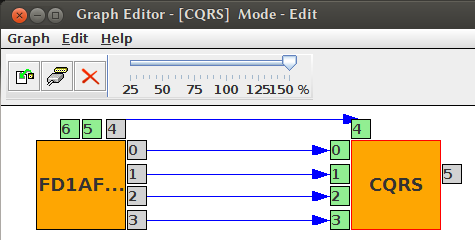
\includegraphics[width=1.0\columnwidth]{images/graph-editor.png}
                \caption{Graph editor of WS-PGRADE}
                \label{fig:grapheditor}
\end{figure*}

\begin{figure*}%[!b]
                \centering
                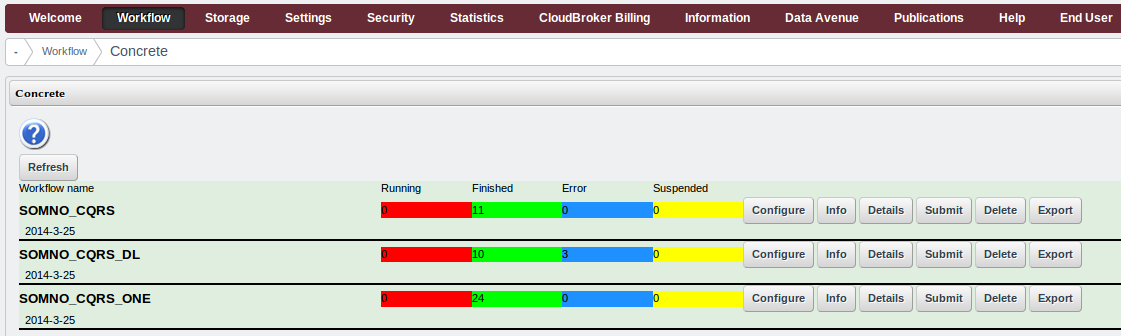
\includegraphics[width=2.0\columnwidth]{images/interface-workflows.png}
                \caption{List of concrete workflows in the web portal}
                \label{fig:interfaceworkflows}
\end{figure*}


\subsection{DCI-Bridge}\label{dci}

The DCI-Bridge is part of gUSE and connects the workflow system with different types of Distributed Computing Infrastructures (DCI).
These middlewares are for example grid or cloud infrastructures, where applications can be executed.
The DCI-Bridge is a generic interface receiving requests from the workflow system.
Different DCI plugins handle these request for different infrastructure types.
To connect a cloud infrastructure the DCI-Bridge provides a CloudBroker and a EC2 plugin.
Cloudbroker is an external service which is used to connect to a cloud.
As the SOMNO.Netz server architecture is encapsulated in a private network, which can not be reached from outside, this is not a suitable option.
Instead the EC2 plugin is being used, which connects to the cloud directly by talking to the EC2 interface of OpenStack (see section~\ref{openstack}), using the opensource command-line software euca-tools.

\subsection{Sample Applications}\label{applications}

TODO

\subsection{Workflow Repositories}\label{repositories}

TODO


\section{Implementation}\label{implementation}

TODO

\subsection{Architecture}\label{architecture}

Installation of gUSE

\begin{figure*}%[!b]
                \centering
                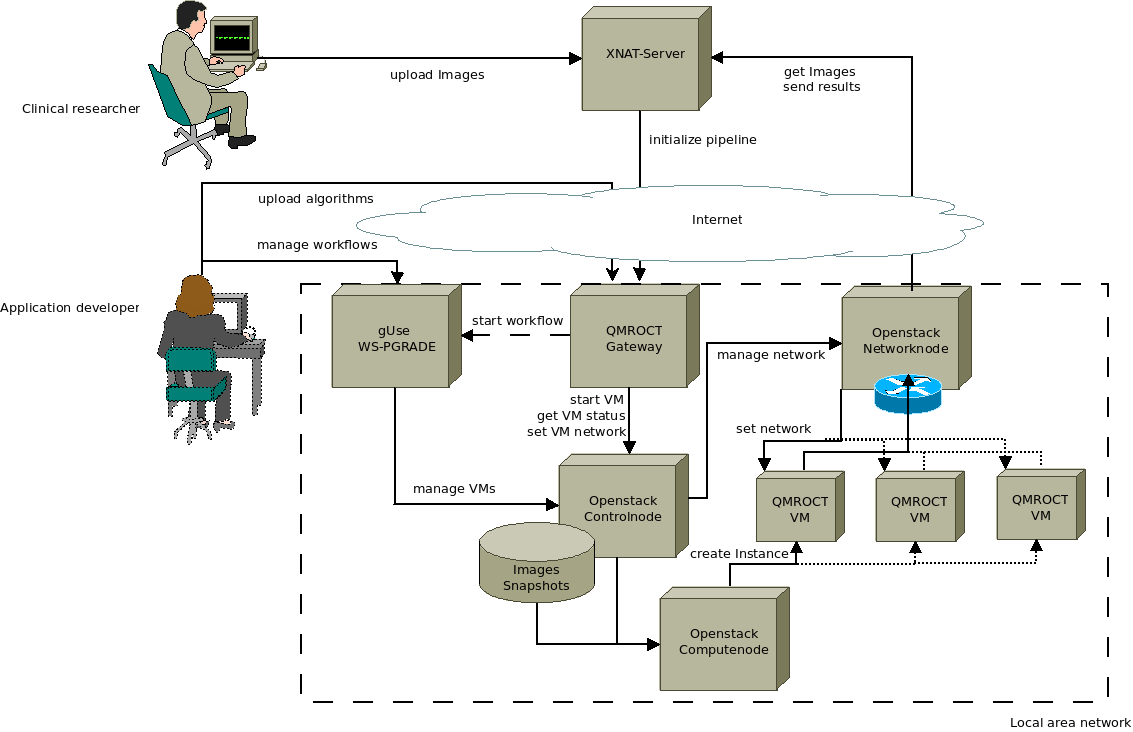
\includegraphics[width=2.0\columnwidth]{images/somno-architecture.png}
                \caption{Architecture of QM-ROCT \cite{wu14} including WS-PGRADE/gUSE}
                \label{fig:architecture}
\end{figure*}

euca tools hack

\subsection{Concrete Workflows}\label{concrete}

How to create

Alternative solutions

\subsection{Remote API}\label{api}

Generally working, but not for cloud

not many control options

research build their own systems on top of java api

processing manager may be an alternative in the future, but adds more overhead


\section{Results}\label{results}

TODO

\subsection{Improvements}\label{improvements}

Can have multiple dependent jobs/algorithms

reusing VMs - closes after some time

\subsection{Problems}\label{problems}

unecessary data copying - not using same VM for followup jobs

no error handling

no or only few information in interface, if problem related to cloud, not application

only few information in log files

manual resume not always helping

sometimes workflows not startable, need to restart gUSE often - unstable

Rest API Generally working, but not for cloud, not many control options, research build their own systems on top of java api, processing manager may be an alternative in the future, but adds more overhead

\subsection{Testing}\label{testing}

starting different tests under different conditions

works with reliable cloud

but not when cloud is busy and may fail

problems with handing data from one job to another with parameter sweep (works with only one job)

\subsection{Missing functionality}\label{missing}

cloud debug -> snapshot

Visualization of running VMs

Information about errors in interface and/or error documentation

more options for controlling the cloud resources

need to restart gUSE when changing stuff

userfriendly interface

option to use the system without the web interface


\section{Discussion}\label{discussion}

WS-PGRADE/gUSE is a workflow management system, that has been used to execute applications in grid infrastructures successfully.
By porting this functionality to a cloud infrastructure new challenges arise for data and error handling.

In the current state WS-PGRADE/gUSE has no cloud specific features.
The data model of sending files between gUSE server and the cloud infrastructure has not been adapted for cloud architectures.
The performance could be improved significantly by reducing the amount of data transfers.
For WS-PGRADE/gUSE the cloud is just another grid and the characteristics of cloud infrastructures are being ignored.

Since gUSE is able to perform a lot of tasks by providing a complex workflow system it would be great to use it in the QMROCT/SOMNO.Netz data processing infrastructure.
Unfortunately gUSE is only as stable as the underlying cloud and not able to handle any errors or delays caused by the cloud.
Therefore the system becomes unreliable.
Furthermore gUSE needs to be restarted as soon as unexpected errors occur.
It is the only way of restoring a stable system environment.

Due to this serious issues it is not possible to use WS-PGRADE/gUSE for a productive cloud-based architecture right now.
In order to improve the system, it is important to further investigate the given issues and to report back to the developers which improvements are necessary before a productive usage is possible.


\end{multicols}

\end{document}